\documentclass[varwidth,convert={density=500,size=1080x800,outext=.png}]{standalone}
\usepackage{mathtools}
\usepackage{graphicx}
\usepackage{bm}
\usepackage{color}
\usepackage[dvipsnames,table]{xcolor}
\usepackage{tikz}
\usepackage{stanli}
\usepackage{verbatim}
\usepackage{tikz}
\usetikzlibrary{shapes,calc,through,3d,patterns}
\usetikzlibrary{decorations.pathreplacing}
\usepackage{pgfplots}
\usepackage{siunitx} % For formatting numbers
\usepackage{hyperref}
\hypersetup{colorlinks=true,linkcolor=darkred}
\usepackage{multicol}
\usepackage[absolute,overlay,]{textpos}
\usepackage{pgfplots}
\pgfplotsset{width=10cm,compat=1.9}
\usepackage{subcaption}
\usepackage{multirow}
\usepackage{bbding}
\usepackage{arydshln}
\usepackage{mathtools}
\usepackage{tcolorbox}

\usepackage[dvipsnames]{xcolor}

\begin{document}
    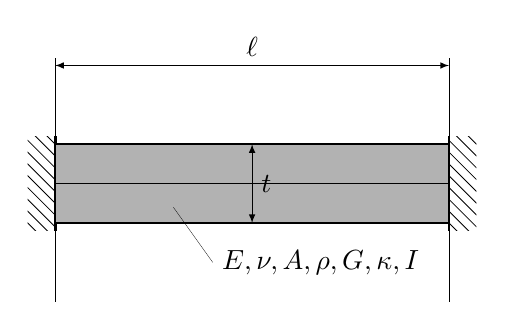
\begin{tikzpicture}
      \point{a}{0}{0};
      \support {3}{a}[270];
      \point{b}{5}{0};
      \support {3}{b}[90];
      % Draw the rectangle
      \filldraw[fill=gray!60, draw=black,thick] (0,-0.5) rectangle (5,0.5);
       %axis
      \draw[ultra thin] (0,0) -- (5,0);
      \draw[ultra thin] (0,-1.5) -- (0,1.6);
      \draw[ultra thin] (5,-1.5) -- (5,1.6);
      % length
      \draw[latex-latex, ultra thin]  (0,1.5)  to node[midway,above] {$\ell$}(5,1.5) ;
      %thick
            \draw[latex-latex, ultra thin]  (2.5,-0.5)  to node[midway,right] {$t$}(2.5,0.5) ;
      \draw[ultra thin]  (1.5,-0.3) -- (2,-1) node[right]{$E,\nu,A,\rho,G,\kappa,I$};
    \end{tikzpicture}
  \end{document}